\documentclass[12pt]{article}
\usepackage{geometry}
\usepackage{amsmath}
\usepackage{amssymb}
\usepackage{enumitem}
\usepackage{fancyhdr}
\usepackage{framed}
\usepackage{tikz}
%\usepackage{charter}
\usepackage{mathpazo}
%\usepackage{newcent}
\usepackage{indentfirst}
\usepackage{booktabs}
\usepackage{graphicx}
\usepackage{float}
\usepackage{makecell}
\usepackage{xcolor}
\usepackage{mdframed}
\usetikzlibrary{trees}
\pagestyle{fancy}
\usepackage{amsthm}
\theoremstyle{definition}
\newtheorem{definition}{Definition}[section]
\theoremstyle{property}
\newtheorem{property}{Property}[section]
\theoremstyle{assumption}
\newtheorem{assumption}{Assumption}[section]
\theoremstyle{example}
\newtheorem{example}{Example}[section]
\theoremstyle{comment}
\newtheorem{comment}{Comment}[section]
\newtheorem{theorem}{Theorem}[section]
\newtheorem{corollary}{Corollary}[theorem]
\newtheorem{lemma}[theorem]{Lemma}
\usepackage{lastpage}
\usepackage{wrapfig}
\usepackage{hyperref}
\usepackage{subcaption}
\usepackage{setspace}
\hypersetup{
colorlinks=true,
linkcolor=black,
filecolor=green, 
urlcolor=blue,
}
\newcommand{\ROM}[1]
    {\MakeUppercase{\romannumeral #1}}
\fancyhead[L]{Econometrics \ROM{2}: Recitation 12 }%change each reci
\fancyhead[R]{Spring 2020}
\fancyfoot[C]{\thepage \hspace{1pt} / \pageref{LastPage}}

\fancypagestyle{firstpage}{%
\fancyhf{}%
\renewcommand{\headrulewidth}{0mm}%
  \fancyfoot[C]{\thepage \hspace{1pt} / \pageref{LastPage}}
}

\usepackage{wrapfig}

\lhead{Introduction to Econometrics}

\rhead{Recitation 5}


\title{Introduction to Econometrics: Recitation 5}

\begin{document}
\linespread{1.25}
\author{Seung-hun Lee}
\date{}
\maketitle

\section{Multivariate Regression Models}

\subsection{Multivariate Regression: Sampling Statistics}
The estimates for the $\hat{\beta}_j, \ j\in\{0,1,2\}$ can be obtained in a similar way in which we have obtained the OLS estimates for the single variable version. Namely, solve the following minimization problem and get first order conditions with respect to $\beta_0, \beta_1, \beta_2$
\[
\min_{\{\beta_0,\beta_1,\beta_2\}} \sum_{i=1}^n[Y_i-\beta_0 - \beta_1X_{1i}-\beta_2X_{2i}]^2
\]
After some more amount of algebra (than the single variable case), the result we get is the following
\begin{itemize}
\item[$\hat{\beta}_0=$] $\bar{Y}-\hat{\beta}_1\bar{X}_1-\hat{\beta}_2\bar{X}_2$
\item[$\hat{\beta}_1=$] $\frac{\sum_{i=1}^n (X_{1i}-\bar{X}_1)(Y_{i}-\bar{Y})\sum_{i=1}^n(X_{2i}-\bar{X}_2)^2-\sum_{i=1}^n (X_{2i}-\bar{X}_2)(Y_{i}-\bar{Y})\sum_{i=1}^n(X_{1i}-\bar{X}_1)(X_{2i}-\bar{X}_2)}{\sum_{i=1}^n (X_{1i}-\bar{X}_1)^2\sum_{i=1}^n (X_{2i}-\bar{X}_2)^2-[\sum_{i=1}^n (X_{1i}-\bar{X}_1)(X_{2i}-\bar{X}_2)]^2}$
\item[$\hat{\beta}_2=$] $\frac{\sum_{i=1}^n (X_{2i}-\bar{X}_2)(Y_{i}-\bar{Y})\sum_{i=1}^n(X_{1i}-\bar{X}_1)^2-\sum_{i=1}^n (X_{1i}-\bar{X}_1)(Y_{i}-\bar{Y})\sum_{i=1}^n(X_{1i}-\bar{X}_1)(X_{2i}-\bar{X}_2)}{\sum_{i=1}^n (X_{1i}-\bar{X}_1)^2\sum_{i=1}^n (X_{2i}-\bar{X}_2)^2-[\sum_{i=1}^n (X_{1i}-\bar{X}_1)(X_{2i}-\bar{X}_2)]^2}$
\end{itemize} \par\medskip
However, what matters at this point is how we should interpret these coefficients. Suppose that we raise the amount of $X_{1i}$ and leave others unchanged. Then $Y_i$ changes by $\hat{\beta}_1$. Therefore, $\hat{\beta}_1$ measures the change in $Y_i$ due to change in $X_{1i}$ \emph{while leaving other independent variables constant} (ceteris paribus). If other variables are allowed to change, then the change in $Y_i$ due to change in $X_i$ by 1 unit is not guaranteed to be equal to $\hat{\beta}_1$.

\subsection{Multicollinearity}
When including more independent variables, we are quite likely to end up including independent variables that are highly correlated with each other. \textbf{Multicollinearity} refers to this situation. There are two types of multicollinearities. We say two variables $X_1$ and $X_2$ are \textbf{perfectly multicollinear} if $X_1$ is in an exact linear relationship of some sort with $X_2$. Any multicollinearities that are not in exact linear relationship is referred to as \textbf{imperfect multicollinearity}. \par\medskip

When there is a perfect multicollinearity, we run in to the situation where the denominator and the numerator of the OLS estimates is not defined. These two cases demonstrate possible consequences of multicollinearity
\begin{itemize}
\item \textbf{Assume that $X_2 = cX_1$ for some constant $c$}: Then we have $(X_{2i}-\bar{X}_2)=c(X_{1i}-\bar{X}_1)$. Then $\hat{\beta}_1$ changes to
\scriptsize{\begin{gather*}
\frac{\sum_{i=1}^n (X_{1i}-\bar{X}_1)(Y_{i}-\bar{Y})c^2\sum_{i=1}^n(X_{1i}-\bar{X}_1)^2-c\sum_{i=1}^n (X_{1i}-\bar{X}_1)(Y_{i}-\bar{Y})c\sum_{i=1}^n(X_{1i}-\bar{X}_1)(X_{1i}-\bar{X}_1)}{\sum_{i=1}^n (X_{1i}-\bar{X}_1)^2 c^2\sum_{i=1}^n (X_{1i}-\bar{X}_1)^2-c^2[\sum_{i=1}^n (X_{1i}-\bar{X}_1)(X_{1i}-\bar{X}_1)]^2} \\
=\frac{0}{0} = ???
\end{gather*}}\normalsize
Therefore, $\hat{\beta}_1$ will not be defined (similar for $\hat{\beta}_2$).
\item \textbf{Dummy variable trap}: Say that you have the dummy variable for females and males. Let each of them be $X_{1i}$ and $X_{2i}$ with $X_{2i}=1-X_{1i}$. Then the regression can be written as
\begin{gather*}
Y_i = \beta_0 + \beta_1X_{1i} + \beta_2X_{2i} + u_i \iff Y_i = \beta_0 + \beta_1X_{1i} + \beta_2(1-X_{1i}) + u_i \\
\iff Y_i = \beta_0 + \beta_2 +(\beta_1-\beta_2)X_{1i}+u_i
\end{gather*}
Therefore, by including both $X_{1i}$ and $X_{2i}$ in the same regression, the $X_{2i}$ vanishes from the equation. This is why when you have dummy variables for all categories in the observation, one of them must be left out.
\end{itemize} \par\medskip
The STATA deals with perfect multicollinearity by dropping out some variables that cause perfect multicollinearity.

%%%%%%%%%%%%%%%%%%
\subsection{Joint testing: Types of Hypothesis Testing}
We have covered hypothesis tests since the beginning of this course. In the regression with single independent variable, we have used $t$-distribution (or if $n$ is sufficiently large, normal distribution) to check whether the following hypothesis hold:
\[
H_0 : \beta_1 = 0 \ \ H_1 : \beta_1 \neq 0
\]
and the test statistic was (assuming homoskedasticity)
\[
t=\frac{\hat{\beta}_1-0}{s.e(\hat{\beta})}\sim t_{n-2} \ \ (\sim N(0,1) \ \text{in large samples})
\]
where $s.e(\hat{\beta}_1)=\sqrt{\frac{1}{n}\frac{\frac{1}{n-2}\sum_{i=1}^n(X_i-\bar{X})\hat{u}_i}{(\frac{1}{n}\sum_{i=1}^n (X_i-\bar{X})^2)^2}}$. So it may seem plausible to think that to test the hypothesis on a setting where we have multiple independent variables, we just need to run this many times. However, this is not exactly the case. the following example demonstrates why. \\ \par

\begin{mdframed}[backgroundcolor=blue!5] 
\textbf{Why do multiple testing using $t$-statistics have problems?} \medskip \\ 
Consider the case where there is you are testing on multiple independent variables. Suppose that you are running a two-sided test with 5 independent variables and significance level $\alpha = 5\%$ under the null hypothesis
\[
H_0: \beta_1=...\beta_5=0
\]
You reject the null hypothesis when $|t_i|\geq 1.96 \ i\in\{1,2,3,4,5\}$ Note that for each $i$, the probability of $|t_i|\geq 1.96$ is 0.05. Now assume that each test statics are independent. Then the probability of incorrectly rejecting the null hypothesis using this approach is
\[
\begin{aligned}
\Pr(|t_1|>1.96 \cup...\cup |t_5|>1.96) & =1-\Pr(|t_1|\leq1.96\cap .. \cap|t_1|\leq1.96)\\
(\because\text{Independence of $t_i$'s}) \ \ &=1-\Pr(|t_1|\leq1.96)\times ..\times\Pr(|t_5|\leq1.96) \\
 & = 1-(0.95)^5 \\
 &= 0.2262
\end{aligned}
\]
This means that the rejection rate under the null is not 5\% but 22\% percent. Therefore, we end up rejecting the null hypothesis more than we have to. (Formally, we say that the probability of type 1 error rises sharply.) 
\end{mdframed} \par\medskip
Because of this fact, we require another approach when testing multiple hypotheses at the same time. This is where \textbf{$F$-test} comes in. This is a test where all parts of the joint hypothesis can be tested at once. It also has mechanism for correcting the correlation between the $t$-test statistics. It ultimately allows us to correctly set the significance level even for the multiple testing case. \par\medskip
The usual joint hypothesis test for the regression with $k$ variables (not including the constant term) is
\[
H_0: \beta_1 = ... =\beta_k=0, \ H_1:\lnot H_0
\]
where $H_1$ refers to the case where there is a nonzero element in any one of $\beta_1$ to $\beta_k$. The $\lnot$ symbol refers to ``not". Note that the default F-test null hypothesis for STATA is $H_0:\beta_1 = ... =\beta_k=0$ and $H_1: \lnot H_0$.\par\medskip
We can actually go farther. Suppose that instead of $\beta_1$ and $\beta_2$ being zero, we are just interested in whether they are equal. The $F$-test can also be used for testing this hypothesis. The setup of the hypothesis would be
\[
H_0: \beta_1 = \beta_2 \ H_1: \beta_1 \neq \beta_2
\]
I will discuss how to implement such hypothesis test on STATA in the next section. \par\medskip
\noindent
\textit{For curious minds: } Note that the square of the $t$ distribution with the degree of freedom $n$ is equivalent to the $F$ distribution with $1$ degree of freedom in the numerator and $n$ in the denominator. For more information, please refer the link I attach in the footnotes\footnote{\url{http://homepage.stat.uiowa.edu/~rdecook/stat3200/notes/t_and_F_4pp.pdf}}
\subsection{Interpreting the Results}
Below are the results of a regression on multiple variables. I am using the data from Professor Almond's paper on cost of low birthweight\footnote{Almond, Douglas, Kenneth Chay, David Lee (2005) ``The Costs of Low Birthweight", \textit{Quarterly Journal of Economics} 120(3):1031-1083}. I regress \textit{birthweight} on \textit{smoker, alcohol, Nprevist} (number of prenatal visits to doctor).
\begin{figure}[H]
\begin{center}
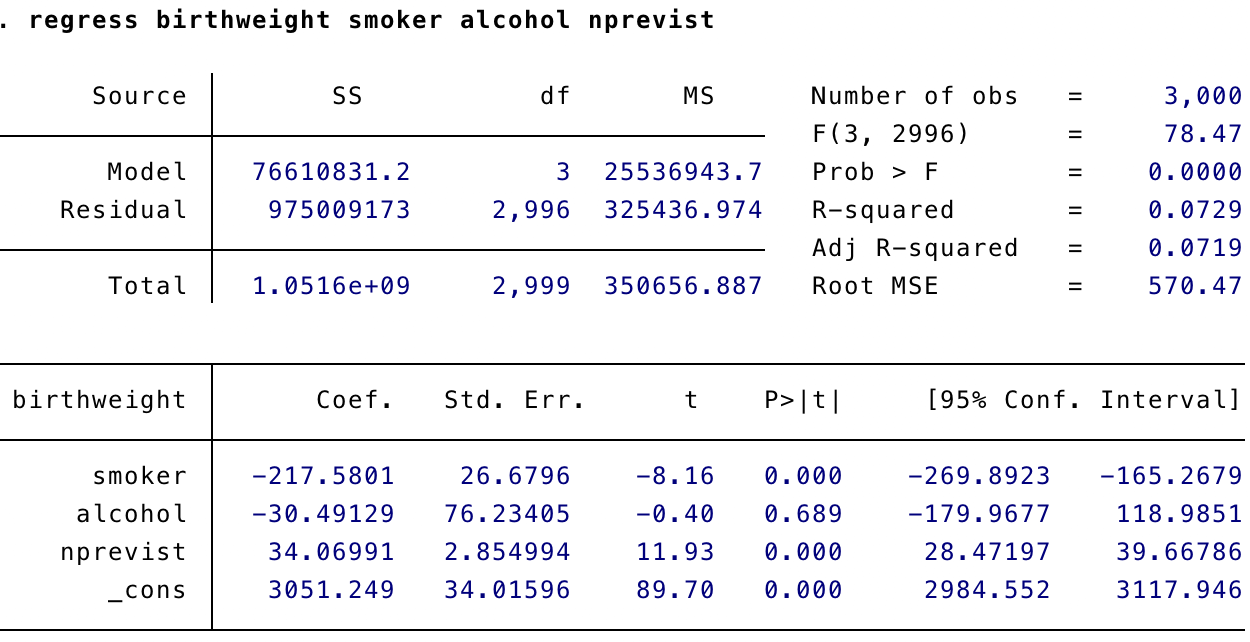
\includegraphics[width=0.7\textwidth]{regoutput.png}
\end{center}
\end{figure}\par\medskip
You can see that running multivariate regression is similar in terms of the techniques involved. Additional complication rises from interpreting the goodness of fit. In addition to $R^2$, we now get the \textbf{adjusted $R^2$}, which is defined as
\[
\bar{R}^2 = 1-\frac{n-1}{n-k-1}\frac{\text{Residual Sum of Squares}}{\text{Total Sum of Squares}}
\]
Since we are assuming that $k\geq 1$, adjusted $R^2$ is smaller than the $R^2$. As we include more variables, the $\frac{n-1}{n-k-1}$ increases, leading to further decrease in adjusted $R^2$. However, if the new variables are very relevent, $\frac{\text{Residual Sum of Squares}}{\text{Total Sum of Squares}}$ decreases. This reduces the gap between $R^2$ and the adjusted $R^2$. If the adjusted $R^2$ do not decrease drastically, it is a sign that we are adding a relevant variable. \par\medskip
One way to conduct various hypothesis testing is to utilize the \texttt{test} command. I include two pictures, one with $H_0: \beta_{\text{smoker}}=\beta_{\text{alcohol}}=\beta_{\text{nprevist}}=0$ on the left and the other with $H_0:\beta_{alcohol}+\beta_{nprevist}=0$ on the right.
\begin{figure}[H]
\begin{center}
        \begin{subfigure}[b]{0.45\textwidth}
	\centering
                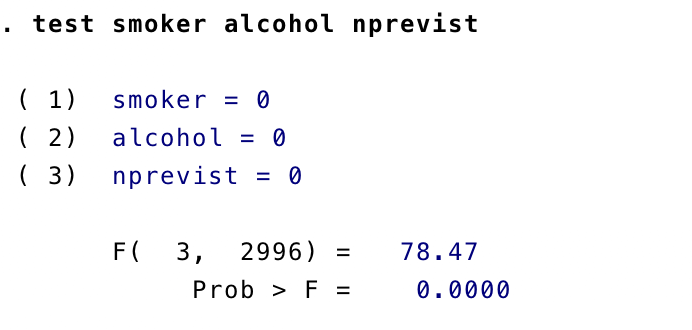
\includegraphics[width=\linewidth]{test}
        \end{subfigure}
        \begin{subfigure}[b]{0.45\textwidth}
	\centering
                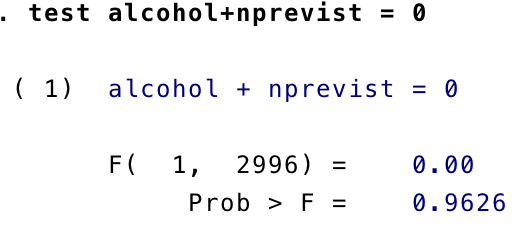
\includegraphics[width=\linewidth]{test1}
        \end{subfigure}
\end{center}
\end{figure}



%%%%%%%%%%%%%%%%%%
\subsection{F-tests}
You should know after the problem sets that you use $F$-tests to assess the results of a joint hypothesis. The \textbf{$F$-statistics} are calculated in two ways. One uses $t$-statistics from individual hypotheses. This is calculated as
\[
\frac{1}{2}\left(\frac{t_1^2+t_2^2-2\hat{\rho}_{t_1,t_2}t_1t_2}{1-\hat{\rho}^2_{t_1,t_2}}\right)
\]\par\medskip
Another one, which is useful for calculating $H_0: \beta_1 = ... =\beta_q=0$ hypothesis ($q$ is the number of hypotheses being tested on) uses $R^2$ from the 'unrestricted' and 'restricted' regressions. Assume that there are total of $k$ independent variables, where $k\geq q$ and the null hypothesis is as stated above. The restricted regressions and unrestricted regressions are defined as
\[\begin{aligned}
\text{Restricted: } & Y_i =\beta_0+ 0X_{1,i} + ...+ 0X_{q,i}+ \beta_{q+1}X_{q+1,i}+...+\beta_kX_{k,i} + u_i\\
\text{Unrestricted: } & Y_i = \beta_0+\beta_1X_{1,i} + ... +\beta_qX_{q,i}+ \beta_{q+1}X_{q+1,i}+...+\beta_kX_{k,i} + u_i\\
\end{aligned}\] \par\medskip
You can now notice that restricted regression assumes that $H_0$ is true and then only optimizes with respect to $\beta_{q+1},...,\beta_{k}$. Unrestricted regression does not assume that $H_0$ is true and optimizes with respect to all slope coefficients. The second formula for $F$-statistic uses $R^2$ from these two regressions. Intuitively, the unrestricted regression allows for the role of $X_1,..,X_q$ whereas their role in restricted regression is limited. This is why $R^2$ in unrestricted regression is higher than restricted regression. Given this, $F$-statistic is
\[
\frac{(R^2_{\text{Unrestricted}}-R^2_{\text{Restricted}})/q}{(1-R^2_{\text{Unrestricted}})/(n-k-1)}
\]
where $k$ is total number of independent variables (not counting intercept) and $q$ is the number of restrictions. \par\medskip
There is another way to express this. Note that $R^2_{\text{Restricted}} = 1-\frac{RSS_{\text{Restricted}}}{TSS}$. $R^2_{\text{Unrestricted}}$ is defined similarly. By using this and with little algebra, we can derive this formula, which is mentioned in most econometrics textbooks.
\[
\frac{(RSS_{\text{Restricted}}-RSS_{\text{Unrestricted}})/q}{(RSS_{\text{Unrestricted}})/(n-k-1)}
\] \par\medskip


\subsection{Control variables and conditional mean independence}
Assume that we have a following setup:
\[
\begin{aligned}
\text{True: }& Y_i = \beta_0 + \beta_1 X_i + \beta_2 Z_i+u_i\\
\text{Mistake: }& Y_i = \beta_0 + \beta_1 X_i + u_i^*\\
\text{Sample: }& Y_i = \hat{\beta}_0 + \hat{\beta}_1 X_i+ \hat{u}_i\\
\end{aligned}
\]
If we end up with an omitted variable bias by not including $Z_i$, Then, we have a problem. We can see this from
\[
\begin{aligned}
E[u_i^*|X_i]&=E[\beta_2Z_i+u_i|X_i]\\
&=\beta_2Z_i+E[u_i|X_i] \neq 0
\end{aligned}
\]
So Assumption 2 from the classical linear regression model (refer to Recitation 3), fails and $\hat{\beta}_1$ without inclusion of $Z_i$ is biased. To address this, we ideally add this variable into the regression. That may not always be possible. In that case, we can find $W_i$ variable that is correlated with $Z_i$ to some extent and include that in the regression. By doing so, we achieve three things
\begin{itemize}
\item The $u_i$ term is no longer correlated with $X_i$ ($cov(X_i, u_i)=0$)
\item For given value of $W_i$, then the variable of interest $X_i$ is no longer correlated with the omitted determinant of $Y_i$
\item For given $W_i$, $X_i$ acts as if they are randomly assigned
\end{itemize}
Variable $W_i$ that achieves this is called an \textbf{effective control variable}. In this particular case, we say that the \textbf{conditional mean independence} hold, in the sense that as long as we control for $W_i$, $u_i$ is independent of $X_i$ - making our coefficient of interest unbiased. 
\[
E[u_i|X_i,W_i]= E[u_i|W_i]
\]
Note that $W_i$ itself does not need to have causal relationship with $Y_i$
%%%%%%%%%%%%%%%%%%
\section{Nonlinear regressors}
Not everything in real life is correlated in a linear fashion. For instance, production function are not usually linear with respect to its inputs (Cobb-douglas production function), Wage rises, but the rate at which it rises falls over time (Mincer equation, from Mincer (1974)\footnote{\scriptsize{Mincer, Jacob (1974) "Schooling, Experience, and Earnings", New York, National Bureau of Economic Research}}), and the effect of classroom size can differ depending on how many students are in the class to begin with(Lazear(2001)\footnote{\scriptsize{Lazear, Edward (2001) "Educational Production", \textit{Quarterly Journal of Economics}, 116(3): 777-803}}). \par\medskip
For correlations like this, resorting to linear regressors would not allow the regression model to have the best fit. This is where the nonlinear regressors come in. Regressions with nonlinear regressors allow us to graph relationship between our $Y$ variable and our $X$ variable that is not necessarily linear. When incorporating such regressors, the interpretation of each coefficient becomes trickier. In the next few subsections, I will walk through implementing and interpreting coefficients for regressors that are not linear. \par\medskip
\subsection{Quadratic terms}
Recall from the regression with single independent variable $Y= \beta_0 + \beta_1X_1+u$, $\beta_1$ coefficient means the marginal effect of $X_1$ on $Y$. Mathematically, there are two ways to show this. (For now, all usual assumptions hold)
\begin{itemize}
\item \textbf{Derivatives}: Take derivatives on $Y$ with respect to $X_1$, this gets us
\[
\frac{\partial Y}{\partial X_1} = \frac{\partial}{\partial X_1}[ \beta_0 + \beta_1X_1+u ] = \beta_1
\]
Given that the idea of derivatives captures how much our $Y$ variable changes with unit change in $X_1$, $\beta_1$ represents how much $Y$ responds to a one unit change in $X_1$
\item\textbf{Taking Differences}: Suppose that you raise the amount of $X_1$ by $\Delta x$. Now the change in the  amount of $Y$, denoted as $\Delta y$, as a result of this change is
\[
\beta_0 + \beta_1(X_1+\Delta x)+u = Y+\Delta y
\] 
By subtracting $Y= \beta_0 + \beta_1X_1+u$, I get
\[
\Delta y = \beta_1 \Delta x \implies \frac{\Delta y}{\Delta x} = \beta_1
\]
\end{itemize} \par\medskip
In this example, the marginal effect of $X$ on $Y$ is constant - it does not depend on $X$! However, there are many relationships that cannot be explained this way. For instance, it is most likely the case that the wage rises with age. However, they are not likely to be in a linear relationship. As one gets older, the rate at which wage increases with age decreases. This is where \textbf{polynomial regressors} can improve the fitting of the regression model. Let wage be $W$ and age be $X$. I now regress the following model.
\[
W = \beta_0 + \beta_1 X+ \beta_2 X^2+u
\]
Then, the marginal impact of age on wage can be captured by
\[
\frac{\partial W}{\partial X} = \beta_1 + 2\beta_2 X
\]\par\medskip
Note now that unlike before, there is a term that depends on $X$. This implies that the marginal effect of age on wage now is different depending on what $X$ variables we use (or age). When $\beta_2$ is positive (negative), then marginal impact of age on wage is higher (lower) for older people. Simply put, age rises at faster (slower) rate for older people. \par\medskip
\end{document}

